%%%==============BT_1==============%%%
\begin{bt}%[0D3H1-4]%[0D7V2-2]%[Dự án đề kiểm tra Toán khối 10 GK2 NH23-24 - Dot 13 - Thái Bảo]%[THPT Rạch Kiến - Tỉnh Long An]
	\begin{enumerate}
		\item Cho hàm số $y=f(x)$ có đồ thị như hình vẽ. Lập bảng xét dấu của $f(x)$.
		\begin{center}
			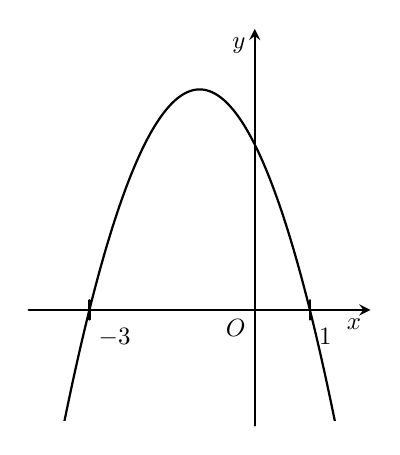
\begin{tikzpicture}[line join=round, line cap=round,>=stealth,thick,scale=.7]
				\tikzset{every node/.style={scale=0.9}}
				\draw[->] (-4.1,0)--(2.1,0) node[below left] {$x$};
				\draw[->] (0,-2.1)--(0,5.1) node[below left] {$y$};
				\draw (0,0) node [below left] {$O$};
				\foreach \x/\nx in {-3/-3,1/1}
				\draw [thick] (\x,5pt)--(\x,-5pt) node [below right] {$\nx$};
				\begin{scope}
					\clip (-4,-2) rectangle (2,5);
					\draw[samples=200,domain=-3.5:1.5,smooth,variable=\x] plot (\x,{-1*(\x)^2+-2*(\x)+3});
				\end{scope}
			\end{tikzpicture}
		\end{center}
		\item Giải bất phương trình $x^2-8x+16\le 0$.
	\end{enumerate}
	\loigiai{
		\begin{enumerate}
			\item Với hàm số $y=f(x)$ có đồ thị như hình vẽ. Ta lập được bảng xét dấu sau
			\begin{center}
				
\begin{tikzpicture}
					\tkzTabInit[deltacl=0.5,espcl=2.5,lgt=2]
					{$x$/1,$f(x)$/1}
					{$-\infty$,$-3$,$1$,$+\infty$}
					\tkzTabLine{,-,0,+,0,-,}
				\end{tikzpicture}
			\end{center}
			\item Tam thức $f(x)=x^2-8x+16$ có $\Delta=0$, hệ số $a=1>0$ nên $f(x)$ luôn dương (cùng dấu với $a$) với mọi $x\neq 4$. Tức là $x^2-8x+16 \geq  0$ với mọi $x$.\\
			Vậy tập nghiệm của bất phương trình là $S=\left\lbrace 4  \right\rbrace$.
		\end{enumerate}
	}
\end{bt}

%%%==============BT_2==============%%%
\begin{bt}%[0D7V3-1]%[Dự án đề kiểm tra Toán khối 10 GK2 NH23-24 - Dot 13 - Thái Bảo]%[THPT Rạch Kiến - Tỉnh Long An]
	Giải phương trình $\sqrt{x^2+3x+1}=\sqrt{3x^2+6x-4}$.
	\loigiai{
		Ta có
		\begin{eqnarray*}
			&	&\sqrt{x^2+3x+1}=\sqrt{3x^2+6x-4} \quad (*)\\
			&\Rightarrow	& x^2+3x+1=3x^2+6x-4\\
			&\Rightarrow	&-2x^2-3x+5=0\\
			&\Rightarrow	& \hoac{	&x=1\\
				&x=\dfrac{-5}{2}.}
		\end{eqnarray*}
		Thay lại hai giá trị của $x$ vừa tìm được vào phương trình $(*)$. Ta thấy $x=-\dfrac{5}{2}$ và $x=1$ đều thỏa mãn.\\
		Vậy tập nghiệm của phương trình là $S=\left\{{-\dfrac{{5}}{2}; 1} \right\}$.
		
	}
\end{bt}

%%%==============BT_3==============%%%
\begin{bt}%[0D8V3-2]%[Dự án đề kiểm tra Toán khối 10 GK2 NH23-24 - Dot 13 - Thái Bảo]%[THPT Rạch Kiến - Tỉnh Long An]
	Khai triển biểu thức $(3x-4)^5$.\\
	\loigiai{
		Thay $a=3x$, $b=-4$ trong công thức khai triển của $(a+b)^5$ ta được
		\begin{eqnarray*}
			(3x-4)^5	&=	& (3x)^5+5\cdot (3x)^4\cdot (-4)^1+10\cdot(3x)^3\cdot(-4)^2+10\cdot(3x)^2 (-4)^3\\
			&	&+5\cdot(3x)^1\cdot(-4)^4+(-4)^5\\
			&=	&243x^5-1620x^4+4320x^3-5760x^2+3840x-1024.
		\end{eqnarray*}
		
	}
\end{bt}

%%%==============BT_4==============%%%
\begin{bt}%[0D8V2-3]%[Dự án đề kiểm tra Toán khối 10 GK2 NH23-24 - Dot 13 - Thái Bảo]%[THPT Rạch Kiến - Tỉnh Long An]
	Cho tập hợp $X=\{1;2;3;4;5\}$.
	\begin{enumerate}
		\item Có bao nhiêu tập con gồm ba phần từ của $X$?
		\item Có thể lập được bao nhiêu số tự nhiên có $4$ chữ số khác nhau từ tập $X$?
	\end{enumerate}
	\loigiai{
		\begin{enumerate}
			\item Số tập con gồm $3$ phần tử của $X$ là tổ hợp chập $3$ của $5$ phần tử $C^3_5=10$.\\
			Vậy có $10$ tập con của $X$ có $3$ phần tử.
			\item Gọi $\overline{a_1a_2a_3a_4}$ là số tự nhiên gồm $4$ chữ số khác nhau từ tập $X$.
			\begin{itemize}
				\item Chữ số $a_1$ có $5$ cách chọn.
				\item Chữ số $a_2$ có $4$ cách chọn.
				\item Chữ số $a_3$ có $3$ cách chọn.
				\item Chữ số $a_4$ có $2$ cách chọn.
			\end{itemize}
			Áp dụng quy tắc nhân ta có $5\cdot 4\cdot3\cdot2=120$.\\
			Vậy có thể lập được $120$ số tự nhiên có $4$ chữ số khác nhau từ tập $X$.
		\end{enumerate}
	}
\end{bt}

%%%==============BT_5==============%%%
\begin{bt}%[0D0H1-2]%[0D0V2-2]%[Dự án đề kiểm tra Toán khối 10 GK2 NH23-24 - Dot 13 - Thái Bảo]%[THPT Rạch Kiến - Tỉnh Long An]
	\begin{enumerate}
		\item Tung một đồng xu cân đối và đồng chất $3$ lần liên tiếp. Hãy xác định không gian mẫu.
		\item Gieo hai con xúc xắc cân đối và đồng chất. Tính xác suất của biến cố $A$: \lq\lq Tổng số chấm trên hai mặt xuất hiện bằng $5$\rq\rq.
	\end{enumerate}
	\loigiai{
		\begin{enumerate}
			\item Không gian mẫu $\Omega=\{SSS;SSN;SNS;SNN;NNN;NSN;NSS;NNS\}$.
			\item Số phần tử $n(\Omega)=6\cdot 6=36$.\\
			Ta có biến cố $A=\{(1;4);(2;3);(3;2);(4;1)\}$.\\
			Suy ra số phần tử biến cố $A$ là $n(A)=4$.\\
			Xác suất biến cố $A$ là $P(A)=\dfrac{n(A)}{n(\Omega)}=\dfrac{4}{36}=\dfrac{1}{9}$.
		\end{enumerate}
	}
\end{bt}

%%%==============BT_6==============%%%
\begin{bt}%[0D0V2-3]%[0D8V2-5]%[Dự án đề kiểm tra Toán khối 10 GK2 NH23-24 - Dot 13 - Thái Bảo]%[THPT Rạch Kiến - Tỉnh Long An]
	\begin{enumerate}
		\item Có bao nhiêu cách chia hết $4$ đồ vật khác nhau cho $3$ người, biết rằng mỗi người nhận ít nhất một đồ vật.
		\item Các bạn An, Bình và $4$ bạn nữa xếp ngẫu nhiên thành một hàng ngang. Tính xác suất để An và Bình đứng ở hai đầu hàng.
	\end{enumerate}
	\loigiai{
		\begin{enumerate}
			\item Do mỗi người nhận ít nhất $1$ đồ vật nên trong $3$ người có: $2$ người nhận $1$ đồ, $1$ người nhận $2$ đồ.
			\begin{itemize}
				\item Chọn $2$ đồ vật từ $4$ đồ vật ta có $C^2_4=6$ cách chọn.
				\item Hoán vị đồ vật cho $3$ người ta có $3!=6$ cách.
			\end{itemize}
			Áp dụng quy tắc nhân ta có $6\cdot 6=36$ cách chia hết $4$ đồ vật khác nhau cho $3$ người, biết rằng mỗi người nhận ít nhất một đồ vật.
			
			\item
			An, Bình và $4$ bạn nữa xếp ngẫu nhiên thành một hàng ngang nên số phần tử không gian mẫu là $n(\Omega)=6!=720$.\\
			Gọi $A$ là biến cố \lq\lq An và Bình đứng ở hai đầu hàng \rq\rq.\\
			Hoán vị vị trí của An và Bình ta có $2!=2$ cách.\\
			Hoán vị vị trí của 4 bạn ở giữa An và Bình ta có $4!=24$ cách\\
			Áp dụng quy tắc nhân ta có $2!\cdot4!=2\cdot 24=48$ cách.\\
			Vậy số phần tử biến cố $A$ là $n(A)=48$.\\
			Xác suất biến cố $A$ là $P(A)=\dfrac{n(A)}{n(\Omega)}=\dfrac{48}{720}=\dfrac{1}{15}$.
		\end{enumerate}
	}
\end{bt}
%%%%%%%%%%%%%%%%%%% Câu 7
	\begin{bt}%[0H9V3-5]%[Dự án đề kiểm tra Toán khối 10 GK2 NH23-24 - Dot 13 - Đình Trí]%[THPT Rạch Kiến - Tỉnh Long An]
	Cho điểm $M(-1;2)$ và đường thẳng $\Delta\colon 4x-3y-5=0$.
	\begin{listEX}
		\item Tính khoảng cách từ điểm $M$ đến đường thẳng $\Delta$.
		\item Lập phương trình tham số của đường thẳng $d$ đi qua điểm $M$ và vuông góc với $\Delta$.
	\end{listEX}
	\loigiai{
		\indent
		Xét điểm $M(-1;2)$ và đường thẳng $\Delta\colon 4x-3y-5=0$.
		\begin{listEX}
			\item Ta có $\mathrm{d}(M,\Delta)=\dfrac{\big|4(-1)-3\cdot 2-5\big|}{\sqrt{4^2+(-3)^2}}=3$.
			\item Gọi $d$ là đường thẳng đis qua điểm $M(-1;2)$ và vuông góc với $\Delta\colon 4x-3y-5=0$.\\
			Khi đó $d$ nhận véc-tơ pháp tuyến $\vec{n}_{\Delta}$ của $\Delta$ làm một véc-tơ chỉ phương.\\
			Do đó $d$ có một véc-tơ chỉ phương $\vec{u}_d=\vec{n}_{\Delta}=(4;-3)$.\\
			Ngoài ra $d$ đi qua điểm $M$ nên phương trình tham số của $d\colon \heva{&x=-1+4t\\&y=2-3t.}$
		\end{listEX}
	}
\end{bt}
%%%%%%%%%%%%%%%%%%% Câu 8
\begin{bt}%[0H9V4-2]%[Dự án đề kiểm tra Toán khối 10 GK2 NH23-24 - Dot 13 - Đình Trí]%[THPT Rạch Kiến - Tỉnh Long An]
	\indent
	\begin{listEX}
		\item Tìm tọa độ tâm $I$ và tính bán kính $R$ của đường tròn $(C)\colon (x-3)^2+(y+4)^2=25$.
		\item Viết phương trình đường tròn $(C')$ có tâm $K(1;-2)$ và đi qua gốc tọa độ $O$.
	\end{listEX}
	\loigiai{
		\indent
		\begin{listEX}
			\item Đường tròn $(C)\colon (x-3)^2+(y+4)^2=25$ có tâm $I(3;-4)$ và bán kính $R=\sqrt{25}=5$.
			\item Đường tròn $(C')$ có tâm $K(1;-2)$ và đi qua $O(0;0)$ có bán kính $R=OK=\sqrt{1^2+(-2)^2}=\sqrt{5}$.\\
			Do đó phương trình đường tròn $(C')\colon (x-1)^2+(y+2)^2=5$.
		\end{listEX}
	}
\end{bt}
%%%%%%%%%%%%%%%%%%% Câu 9
\begin{bt}%[0H9V4-3]%[Dự án đề kiểm tra Toán khối 10 GK2 NH23-24 - Dot 13 - Đình Trí]%[THPT Rạch Kiến - Tỉnh Long An]
	\indent
	\begin{listEX}
		\item Cho tam giác $ABC$, biết $A(-3;0)$, $B(-2;6)$, $C(4;-2)$. Lập phương trình tổng quát của đường trung tuyến $AN$.
		\item Viết phương trình tiếp tuyến của đường tròn $(T)\colon x^2+y^2-2x-4y=0$ tại điểm $E(-1;3)$.
	\end{listEX}
	\loigiai{
		\indent
		Xét $A(-3;0)$, $B(-2;6)$, $C(4;-2)$.
		\begin{listEX}
			\item Trung tuyến $AN$ đi qua trung điểm $N(1;2)$ của cạnh $BC$.\\
			Suy ra $AN$ nhận $\vec{AN}=(4;2)$ và $\vec{u}=(2;1)$ làm các véc-tơ chỉ phương.\\
			Từ đó $AN$ nhận $\vec{n}=(1;-2)$ làm véc-tơ pháp tuyến.\\
			Phương trình tổng quát của $AN\colon 1(x+3)-2(y-0)=0 
			\Leftrightarrow x-2y+3=0$.
			\item Đường tròn $(T)\colon x^2+y^2-2x-4y=0$ có tâm $I(1;2)$ và điểm $E(-1;3) \in (T)$.\\
			Tiếp tuyến của $(T)$ tại $E$ có phương trình
			$$(1+1)(x+1)+(2-3)(y-3)=0 
			\Leftrightarrow 2x-y+5=0.$$
		\end{listEX}
	}
\end{bt}
%%%%%%%%%%%%%%%%%%% Câu 10
\begin{bt}%[0D0C2-6]%[Dự án đề kiểm tra Toán khối 10 GK2 NH23-24 - Dot 13 - Đình Trí]%[THPT Rạch Kiến - Tỉnh Long An]
	\indent
	\begin{listEX}
		\item Một hộp chứa $20$ tấm thẻ có kích thước như nhau và được đánh số từ $1$ đến $20$. Chọn ngẫu nhiên đồng thời $4$ thẻ từ hộp. Tính xác suất để tích các số ghi trên các thẻ chia hết cho $3$.
		\item Một đa giác đều có $2n$ cạnh nội tiếp đường tròn $(O)$. Biết số tam giác tạo thành từ các đỉnh nhiều gấp $20$ lần số hình chữ nhật tạo thành từ các đỉnh. Hỏi đa giác đều đó có tất cả bao nhiêu cạnh?
	\end{listEX}
	\loigiai{
		\indent
		\begin{listEX}
			\item Xét phép thử ``\textit{chọn ngẫu nhiên đồng thời $4$ thẻ từ hộp $20$ thẻ có đánh số từ $1$ đến $20$}''.\\
			Số kết quả có thể xảy ra của phép thử trên là $n(\Omega)=\mathrm{C}_{20}^4$.\\
			Xét biến cố $A$: ``\textit{tích các số ghi trên các thẻ được chọn là một số chia hết cho $3$}''.\\
			$A$ không xảy ra khi ta chọn được cả $4$ thẻ có số trên đó đều không chia hết cho $3$, tức là $4$ số chọn được cùng thuộc tập hợp $\big\{x \in \mathbb{N}^* \mid x \leq 20\big\} \setminus \{3k \mid k \in \mathbb{N}^* \text{ và } k \leq 6\}$.\\
			Do đó, số kết quả thuận lợi cho $A$ là $n(A)=\mathrm{C}_{20}^4-\mathrm{C}_{14}^4$.\\
			Vậy xác suất của biến cố $A$ là $\mathrm{P}(A)=\dfrac{n(A)}{n(\Omega)}=\dfrac{\mathrm{C}_{20}^4-\mathrm{C}_{14}^4}{\mathrm{C}_{20}^4}=\dfrac{3844}{4845}$.
			\item Đường tròn $(O)$ ngoại tiếp đa giác đều $(\mathcal{H})$ $2n$ cạnh có $n$ đường kính đi qua đỉnh của $(\mathcal{H})$.\\
			Mỗi hình chữ nhật lấy đỉnh từ đỉnh của $(\mathcal{H})$ có $2$ đường chéo là $2$ trong $n$ đường kính nêu trên, do đó số hình chữ nhật lấy đỉnh từ đỉnh của $(\mathcal{H})$ là $\mathrm{C}_n^2$.\\
			Cũng từ đỉnh của $(\mathcal{H})$, lập ra các tam giác ta được số tam giác là $\mathrm{C}_{2n}^3$.\\
			Giả thiết bài toán suy ra $\mathrm{C}_{2n}^3=20\mathrm{C}_n^2$ $(n \in \mathbb{N},n \ge 2)$.\\
			Ta có 
			$\begin{aligned}[t]
				\mathrm{C}_{2n}^3=20\mathrm{C}_n^2
				&\Leftrightarrow \dfrac{2n(2n-1)(2n-2)}{3!}=20\cdot\dfrac{n(n-1)}{2!}\\
				&\Leftrightarrow \dfrac{2n(2n-1)(2n-2)}{n(n-1)}=20\cdot\dfrac{3!}{2!}\\
				&\Leftrightarrow 8n-4=60 
				\Leftrightarrow 8n=64
				\Leftrightarrow n=8 \text{ (nhận).}
			\end{aligned}$\\
			Vậy đa giác đều đã cho có $2n=16$ cạnh.
		\end{listEX}
	}
\end{bt}
\Closesolutionfile{ans}

